\documentclass{article}

\usepackage[margin={1in}]{geometry}

\usepackage{tikz}

\usetikzlibrary{arrows.meta,calc,shapes}

\begin{document}
\pagestyle{empty}

\noindent
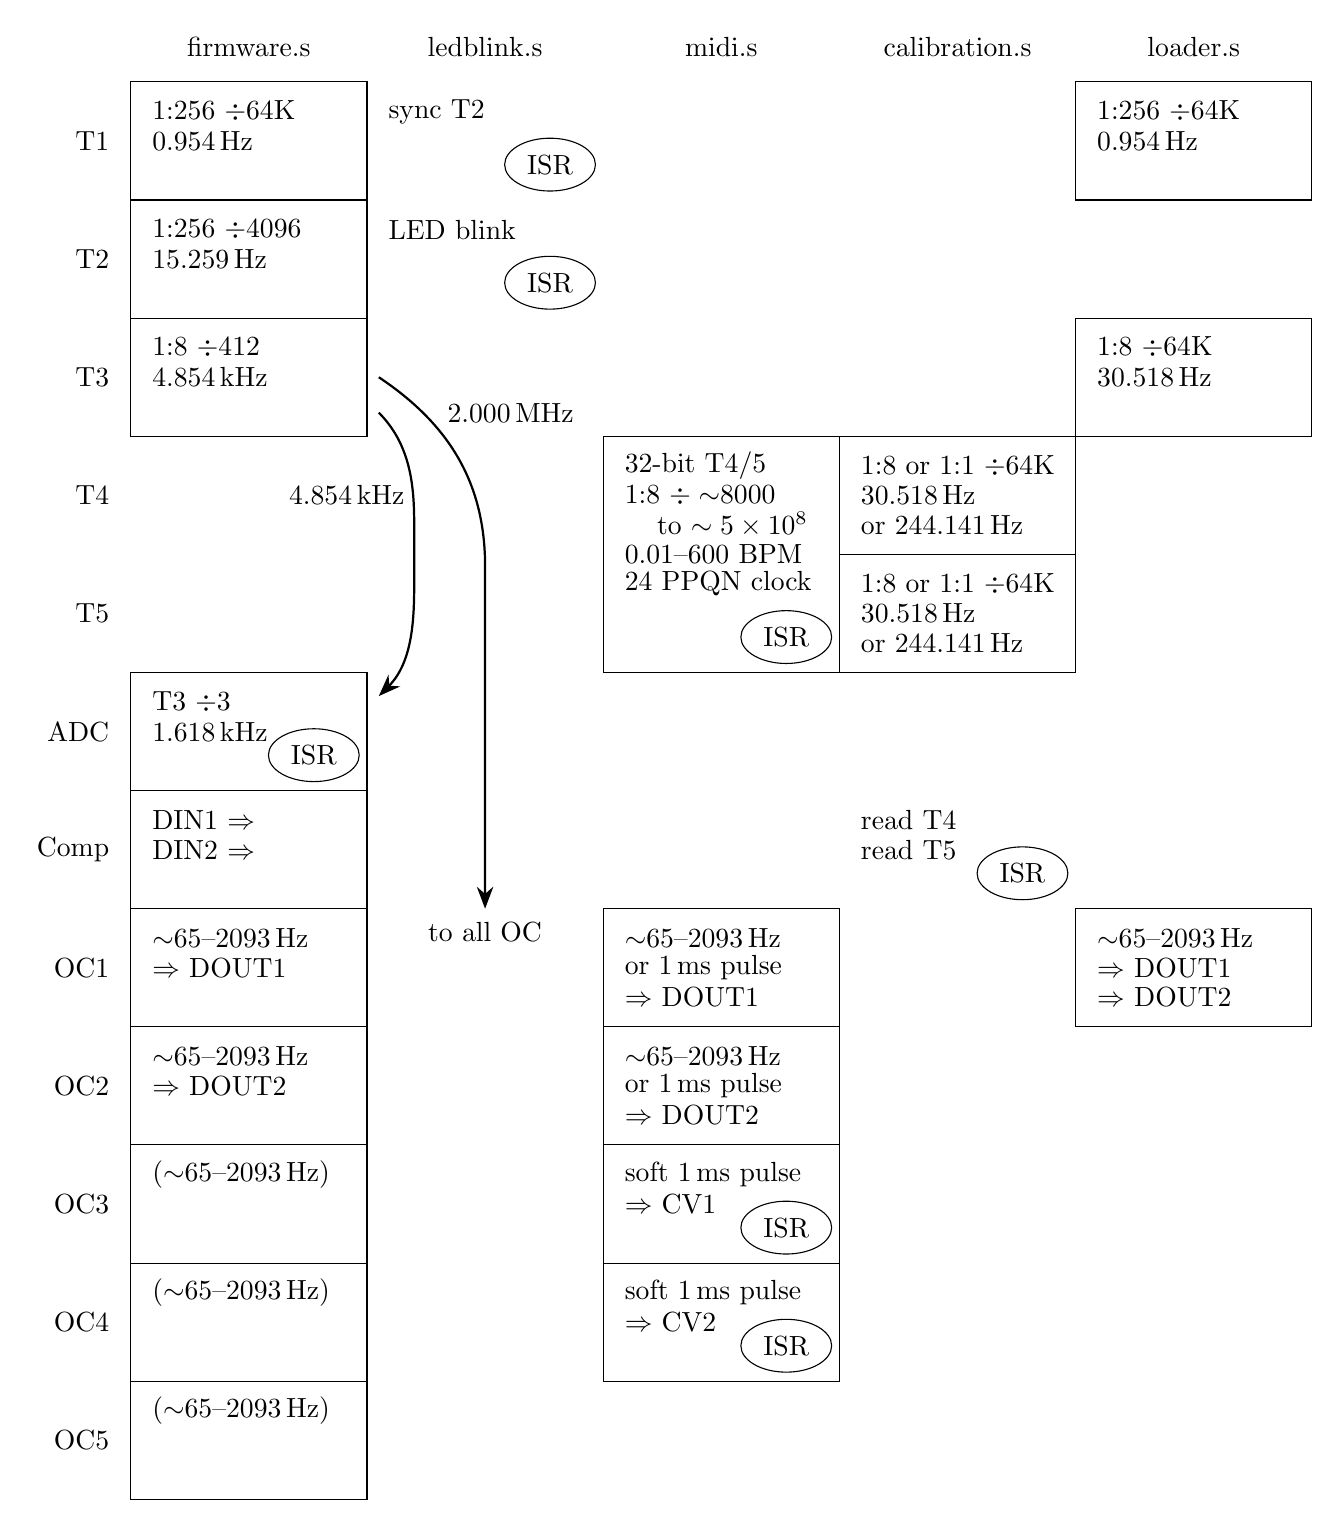
\begin{tikzpicture}[scale=1.5]
  \node at (1,0.3) {firmware.s};
  \node at (3,0.3) {ledblink.s};
  \node at (5,0.3) {midi.s};
  \node at (7,0.3) {calibration.s};
  \node at (9,0.3) {loader.s};
%
  \node[anchor=east] at (-0.1,-0.5) {T1};
  \node[anchor=east] at (-0.1,-1.5) {T2};
  \node[anchor=east] at (-0.1,-2.5) {T3};
  \node[anchor=east] at (-0.1,-3.5) {T4};
  \node[anchor=east] at (-0.1,-4.5) {T5};
  \node[anchor=east] at (-0.1,-5.5) {ADC};
  \node[anchor=east] at (-0.1,-6.5) {Comp};
  \node[anchor=east] at (-0.1,-7.5) {OC1};
  \node[anchor=east] at (-0.1,-8.5) {OC2};
  \node[anchor=east] at (-0.1,-9.5) {OC3};
  \node[anchor=east] at (-0.1,-10.5) {OC4};
  \node[anchor=east] at (-0.1,-11.5) {OC5};
%
  \draw (0,-3) rectangle (2,0);
  \draw (0,-1) -- (2,-1);
  \draw (0,-2) -- (2,-2);
  \draw (8,-1) rectangle (10,0);
  \draw (8,-3) rectangle (10,-2);
  \draw (4,-5) rectangle (8,-3);
  \draw (6,-5) -- (6,-3);
  \draw (6,-4) -- (8,-4);
  \draw (0,-12) rectangle (2,-5);
  \draw (0,-6) -- (2,-6);
  \draw (0,-7) -- (2,-7);
  \draw (0,-8) -- (2,-8);
  \draw (0,-9) -- (2,-9);
  \draw (0,-10) -- (2,-10);
  \draw (0,-11) -- (2,-11);
  \draw (4,-11) rectangle (6,-7);
  \draw (8,-8) rectangle (10,-7);
  \draw (4,-8) -- (6,-8);
  \draw (4,-9) -- (6,-9);
  \draw (4,-10) -- (6,-10);
%
  \node[anchor=west] at (0.1,-0.25) {1:256 $\div$64K};
  \node[anchor=west] at (0.1,-0.5) {0.954\,Hz};
  \node[anchor=west] at (2.1,-0.25) {sync T2};
  \node[anchor=west] at (8.1,-0.25) {1:256 $\div$64K};
  \node[anchor=west] at (8.1,-0.5) {0.954\,Hz};
  \node[anchor=west] at (0.1,-1.25) {1:256 $\div$4096};
  \node[anchor=west] at (0.1,-1.5) {15.259\,Hz};
  \node[anchor=west] at (2.1,-1.25) {LED blink};
  \node[anchor=west] at (0.1,-2.25) {1:8 $\div$412};
  \node[anchor=west] at (0.1,-2.5) {4.854\,kHz};
  \node[anchor=west] at (8.1,-2.25) {1:8 $\div$64K};
  \node[anchor=west] at (8.1,-2.5) {30.518\,Hz};
  \node[anchor=west] at (6.1,-3.25) {1:8 or 1:1 $\div$64K};
  \node[anchor=west] at (6.1,-3.5) {30.518\,Hz};
  \node[anchor=west] at (6.1,-3.75) {or 244.141\,Hz};
  \node[anchor=west] at (6.1,-4.25) {1:8 or 1:1 $\div$64K};
  \node[anchor=west] at (6.1,-4.5) {30.518\,Hz};
  \node[anchor=west] at (6.1,-4.75) {or 244.141\,Hz};
  \node[anchor=west] at (4.1,-3.25) {32-bit T4/5};
  \node[anchor=west] at (4.1,-3.5) {1:8 $\div\sim$8000};
  \node[anchor=west] at (4.1,-3.75) {~~~\,to $\sim5\times10^8$};
  \node[anchor=west] at (4.1,-4.0) {0.01--600 BPM};
  \node[anchor=west] at (4.1,-4.25) {24 PPQN clock};
  \node[anchor=west] at (0.1,-5.25) {T3 $\div$3};
  \node[anchor=west] at (0.1,-5.5) {1.618\,kHz};
  \node[anchor=west] at (0.1,-6.25) {DIN1 $\Rightarrow$};
  \node[anchor=west] at (0.1,-6.5) {DIN2 $\Rightarrow$};
  \node[anchor=west] at (6.1,-6.25) {read T4};
  \node[anchor=west] at (6.1,-6.5) {read T5};
  \node[anchor=west] at (0.1,-7.25) {$\sim$65--2093\,Hz};
  \node[anchor=west] at (0.1,-7.5) {$\Rightarrow$ DOUT1};
  \node[anchor=west] at (4.1,-7.25) {$\sim$65--2093\,Hz};
  \node[anchor=west] at (4.1,-7.5) {or 1\,ms pulse};
  \node[anchor=west] at (4.1,-7.75) {$\Rightarrow$ DOUT1};
  \node[anchor=west] at (8.1,-7.25) {$\sim$65--2093\,Hz};
  \node[anchor=west] at (8.1,-7.5) {$\Rightarrow$ DOUT1};
  \node[anchor=west] at (8.1,-7.75) {$\Rightarrow$ DOUT2};
  \node[anchor=west] at (0.1,-8.25) {$\sim$65--2093\,Hz};
  \node[anchor=west] at (0.1,-8.5) {$\Rightarrow$ DOUT2};
  \node[anchor=west] at (4.1,-8.25) {$\sim$65--2093\,Hz};
  \node[anchor=west] at (4.1,-8.5) {or 1\,ms pulse};
  \node[anchor=west] at (4.1,-8.75) {$\Rightarrow$ DOUT2};
  \node[anchor=west] at (0.1,-9.25) {($\sim$65--2093\,Hz)};
  \node[anchor=west] at (4.1,-9.25) {soft 1\,ms pulse};
  \node[anchor=west] at (4.1,-9.5) {$\Rightarrow$ CV1};
  \node[anchor=west] at (0.1,-10.25) {($\sim$65--2093\,Hz)};
  \node[anchor=west] at (4.1,-10.25) {soft 1\,ms pulse};
  \node[anchor=west] at (4.1,-10.5) {$\Rightarrow$ CV2};
  \node[anchor=west] at (0.1,-11.25) {($\sim$65--2093\,Hz)};
%
  \node[ellipse,draw] at (3.55,-0.7) {ISR};
  \node[ellipse,draw] at (3.55,-1.7) {ISR};
  \node[ellipse,draw] at (5.55,-4.7) {ISR};
  \node[ellipse,draw] at (1.55,-5.7) {ISR};
  \node[ellipse,draw] at (7.55,-6.7) {ISR};
  \node[ellipse,draw] at (5.55,-9.7) {ISR};
  \node[ellipse,draw] at (5.55,-10.7) {ISR};
%
  \draw[thick,-{Stealth[scale=1.2]}]
    (2.1,-2.8) ..controls (2.4,-3.1) and (2.4,-3.5).. (2.4,-3.8)
    -- (2.4,-4.2) ..controls (2.4,-4.5) and (2.4,-4.9).. (2.1,-5.2);
  \draw[thick,-{Stealth[scale=1.2]}]
    (2.1,-2.5) ..controls (2.7,-2.9) and (3.0,-3.4).. (3.0,-4.1)
    -- (3.0,-7.0);
  \node at (3.0,-7.2) {to all OC};
  \node[anchor=east] at (2.4,-3.5) {4.854\,kHz};
  \node[anchor=west] at (2.6,-2.8) {2.000\,MHz};
%  \draw[thick,-{Stealth[scale=1.2]}]
%    (10.1,-2.8) ..controls (10.4,-3.1) and (10.4,-3.5).. (10.4,-3.8)
%    -- (10.4,-6.2) ..controls (10.4,-6.5) and (10.4,-6.9).. (10.1,-7.2);
%  \draw[thick,-{Stealth[scale=1.2]}] (2.7,-6.3)
%    -- (2.7,-7.3) ..controls (2.7,-7.4) and (2.7,-8.0).. (2.1,-8.4);
%  \draw[thick,-{Stealth[scale=1.2]}] (2.7,-7.3)
%    -- (2.7,-8.3) ..controls (2.7,-8.4) and (2.7,-9.0).. (2.1,-9.4);
%  \draw[thick,-{Stealth[scale=1.2]}] (2.7,-8.3)
%    -- (2.7,-9.3) ..controls (2.7,-9.4) and (2.7,-10.0).. (2.1,-10.4);
%  \draw[thick,-{Stealth[scale=1.2]}] (2.7,-9.3)
%    -- (2.7,-10.3) ..controls (2.7,-10.4) and (2.7,-11.0).. (2.1,-11.4);
\end{tikzpicture}

\end{document}
